\documentclass{article}

\usepackage{graphicx}
\usepackage{tikz}
\usepackage{tikzsymbols}
\usetikzlibrary{calc,patterns,shapes.geometric}
\pagestyle{empty}
\usepackage[margin=0pt]{geometry}
\geometry{papersize={14in,12in}}

\def\centerarc[#1](#2)(#3:#4:#5){\draw[#1] ($(#2)+({#5*cos(#3)},{#5*sin(#3)})$) arc (#3:#4:#5);}

\begin{document}
	\begin{figure}
		\centering
		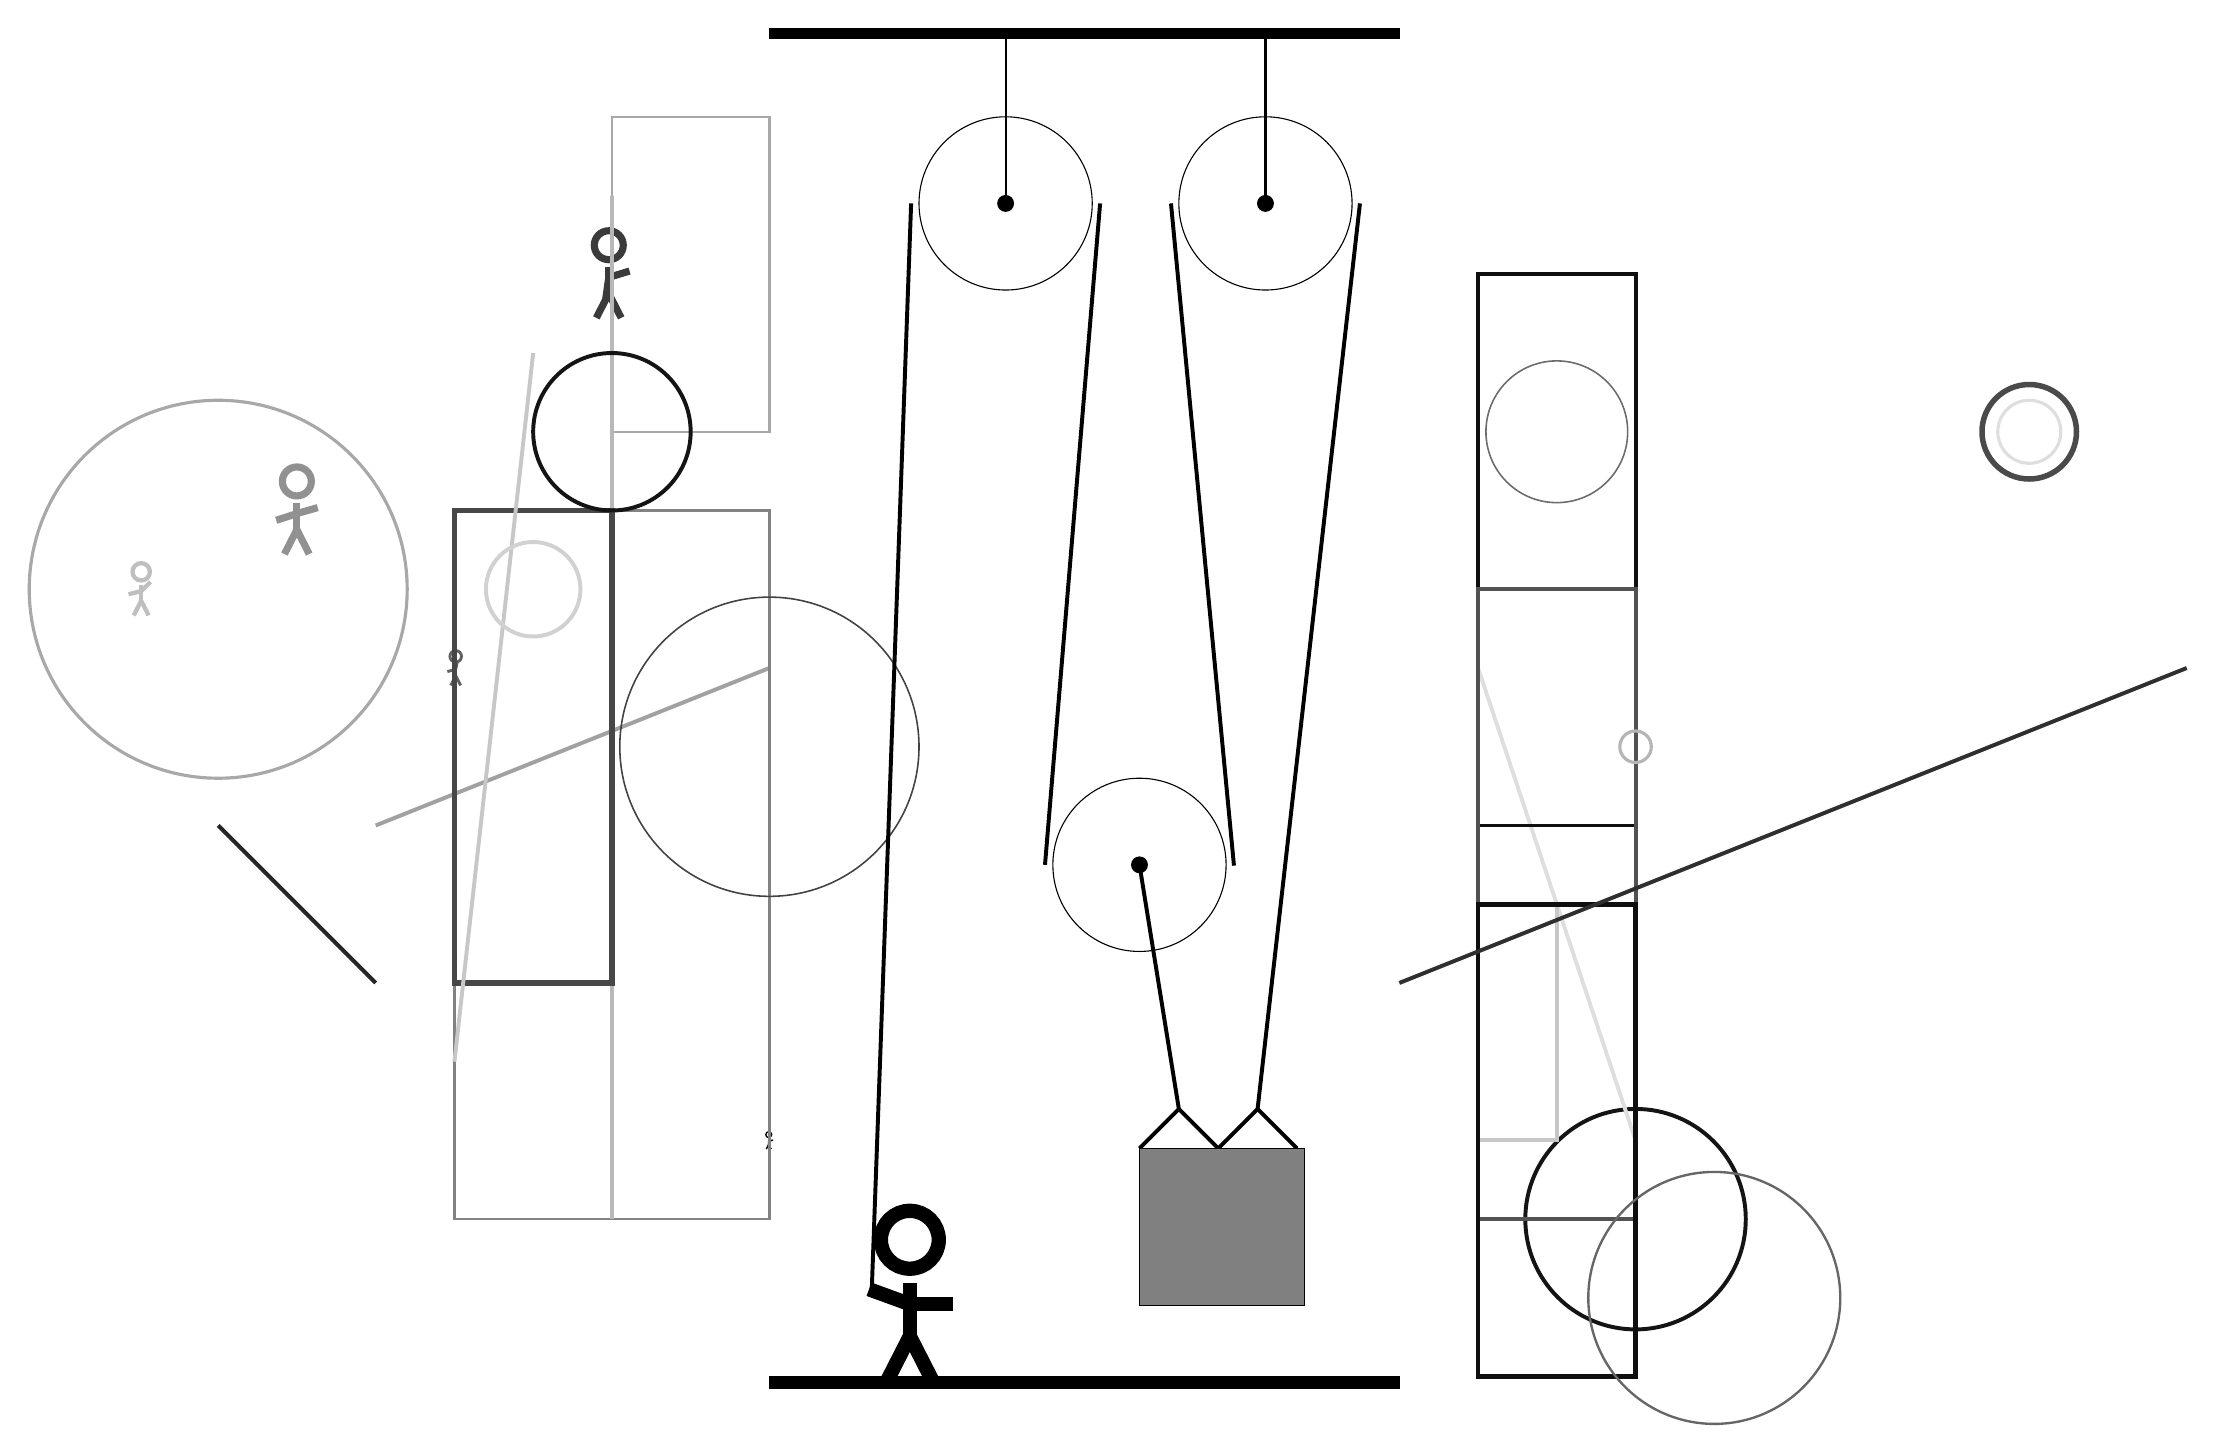
\begin{tikzpicture}
			%%%%% START %%%%%
			
			\draw[fill=black] (-2, 14) rectangle (6, 14.125);
			
			\draw (1, 11.9) circle (1.1);
			\draw[fill=black] (1, 11.9) circle (0.1);
			\draw[thick] (1, 11.9) -- (1, 14);
			
			\draw (4.3, 11.9) circle (1.1);
			\draw[fill=black] (4.3, 11.9) circle (0.1);
			\draw[thick] (4.3, 11.9) -- (4.3, 14);
			
			\draw [line width=0.7mm, color=black!71](14, 9) circle (0.6);
			
			\draw [line width=0.4mm, color=black!34](-9, 7) circle (2.4);
			\draw[line width=0.5mm, color=black!37](-7, 4) -- (-2, 6);
			\draw [line width=0.2mm, color=black!58](8, 9) circle (0.9);
			
			\draw [line width=0.5mm, color=black!92](9, -1) circle (1.4);
			\draw[line width=0.5mm, color=black!13](9, 0) -- (7, 6);
			\node[line width=0.7mm, color=black!25] at (-10, 7) {\Strichmaxerl[3][14][45]};
			\draw[line width=0.5mm, color=black!94] (7, 4) rectangle (9, 11);
			\node[line width=0.6mm, color=black!77] at (-4, 11) {\Strichmaxerl[5][82][17]};
			
			\draw[line width=0.3mm, color=black!34] (-2, 9) rectangle (-4, 13);
			
			\draw [line width=0.4mm, color=black!13](14, 9) circle (0.4);
			
			\node[line width=0.7mm, color=black!95] at (-2, 0) {\Strichmaxerl[1][87][13]};
			\node[line width=0.3mm, color=black!62] at (-6, 6) {\Strichmaxerl[2][16][78]};
			
			\draw[line width=0.3mm, color=black!49] (-2, -1) rectangle (-6, 8);
			\draw[line width=0.5mm, color=black!68] (7, 7) rectangle (9, -1);
			\draw[line width=0.5mm, color=black!22] (8, 0) rectangle (7, 3);
			
			\draw[line width=0.6mm, color=black!94] (7, 3) rectangle (9, -3);
			\draw[line width=0.6mm, color=black!28] (-4, 12) rectangle (-4, -1);
			\node[line width=0.5mm, color=black!43] at (-8, 8) {\Strichmaxerl[5][18][16]};
			
			\draw [line width=0.2mm, color=black!74](-2, 5) circle (1.9);
			\draw[line width=0.7mm, color=black!72] (-4, 2) rectangle (-6, 8);
			\draw [line width=0.3mm, color=black!60](10, -2) circle (1.6);
			
			\draw[line width=0.5mm, color=black!82](6, 2) -- (16, 6);
			\draw [line width=0.4mm, color=black!29](9, 5) circle (0.2);
			\draw [line width=0.5mm, color=black!92](-4, 9) circle (1.0);
			
			\draw[line width=0.5mm, color=black!85](-7, 2) -- (-9, 4);
			
			\draw[line width=0.5mm, color=black!22](-5, 10) -- (-6, 1);
			\draw [line width=0.5mm, color=black!18](-5, 7) circle (0.6);
			
			\draw (2.7, 3.5) circle (1.1);
			\draw[fill=black] (2.7, 3.5) circle (0.1);
			
			\draw[line width=0.5mm]  (2.7, -0.1) -- (3.2, 0.4) -- (3.7, -0.1) -- (4.2, 0.4) -- (4.7, -0.1);
			\draw[fill=black!50] (2.7, -0.1) rectangle (4.8, -2.1);
			
			\draw[line width=0.5mm](-0.7, -1.9) -- (-0.2, 11.9);
			\centerarc[line width=0.5mm](1, 11.9)(0:180:1.2000000000000002);
			\draw[line width=0.5mm](2.2, 11.9) -- (1.5, 3.5);
			\centerarc[line width=0.5mm](2.7, 3.5)(180:370:1.2000000000000002);
			\draw[line width=0.5mm] (3.9, 3.49) -- (3.1, 11.9);
			\centerarc[line width=0.5mm](4.3, 11.9)(0:180:1.2000000000000002);
			\draw[line width=0.5mm](4.2, 0.4) -- (5.5, 11.9);
			\draw[line width=0.5mm] (3.2, 0.4) -- (2.7, 3.5);
			
			\node at (-0.2, -2) {\Strichmaxerl[10][-20][0]};
			
			\draw[fill=black] (-2, -3) rectangle (6, -3.15);
			
			%%%%% END %%%%%
		\end{tikzpicture}
	\end{figure}	
\end{document}